\documentclass[fontsize=13pt,a5paper,twoside, DIV=calc]{scrbook}
\usepackage[ngerman]{babel}

%\usepackage[heuristica,vvarbb,bigdelims]{newtxmath}
\usepackage[T1]{fontenc}
\usepackage{PTSerifCaption} 
%\usepackage[black]{merriweather}

%Erlaubt Einsatz von Farbe
\usepackage[svgnames]{xcolor}
\definecolor{farbe}{HTML}{766D20}
%UTF 8
\usepackage[utf8]{inputenc}
%Schweizer Anführungszeichen
\usepackage[german=swiss]{csquotes}
%Ermöglicht Zierkapitälchen zum Anbsatzanfang
\usepackage{lettrine}
\input Kramer.fd
\renewcommand{\LettrineFontHook}{\color{farbe}\relax\usefont{U}{Kramer}{xl}{n}}
%Um Seitenkopf zu manipulieren
\usepackage{scrpage2}
\pagestyle{scrheadings} 
%Kapitelüberschriften 
%Bilder einbinden
\addtokomafont{chapter}{\Huge\color{farbe}\sffamily}
\usepackage{graphicx}
%Bilder auf ganze Seite ausdehnen
\usepackage{afterpage}
%Bilder von Text umfliessen lassen
%\usepackage[vflt]{floatflt} %vflt=ungerade Seitenzahl Bild rechts und v.v.)
%Für Kapitel Gespenst Jonathan Rahmen ermöglichen
\usepackage[everyline=true]{mdframed}
%Definition Rahmen: links dicker roter balken
\usepackage{tikz} % used for the 'logo' und 
%Abstand zw. Wörtern darf zwecks Blocksatzbildung in Ausnahmefällen bis 1em breit werden.
\setlength{\emergencystretch}{1em}
%Seitenzahlen fett
\addtokomafont{pagenumber}{\bfseries\color{farbe}}
%Satzspiegelberechnung mit allen Parametern nochmals durchführen
\KOMAoptions{DIV=calc}
%Rüschen über Seite
\usepackage{pgfornament}
\chead{\color{farbe}\pgfornament[width=\textwidth,color=farbe]{89}}
%Umkreiste Nummern
\usepackage{circledsteps}

%%%%%%%%%%%%%%%%%%%%%%%%%%%%%%%%%%%%%%%%%%%%%%%%%%%%%%%%%%%%%%%%%%%%%%%%%%%%%%%%%%%%%%%%%%%%%%%%%%%%%%
\begin{document}
%titelseite
%%%%%%%%%%%%%%%%%%%%%%%%%%%%%%%%%%%%%%%%%%%%%%%%%%%%%%%%%%%%%%%%%%%%%%%%%%%%%%%%%%%%%%%%%%%%%%%%%%%%%%
%Kapitel einfügen
\thispagestyle{empty}
\begin{center}

\includegraphics[width=\textwidth]{./bilder/fangen.png}
\end{center}
\vspace*{\fill}
%{\Huge\color{farbe}\hfill{\ttfamily{Fangen}}}
{\centering\fontsize{50}{48} \color{farbe}\sffamily{Fangen}\par}
\addcontentsline{toc}{chapter}{Fangen}
\newpage
%%%%%%%%%%%%%%%%%%%%%%%%%%%%%%%%%%%%%%%%%%%%%%%%%%%%%%%%%%%%%%%%%%%%%%%%%%%%%%%
\lettrine[lines=3, lhang=.2, loversize=.25, lraise=0.05, findent=0.1em,
nindent=0em]{T}{obias} hatte zwei Probleme an diesem Nachmittag. Das erste Problem war eines, ganz nach seinem Geschmack. Jeden Abend hatte er Diskussionen mit seiner Mutter, warum er schon ins Bett musst. Er wollte ihr ganz sachlich erklären, dass Schlafen aber gar nicht nötig sei. Tobias vertraute schon immer der Wissenschaft. Also sass er vor seinem Rechner und suchte das Internet nach Erklärungen ab, warum Menschen – und offensichtlich auch Tiere, schlafen. Verwirrenderweise schien es aber keine echte Erklärung zu geben. Gut, man stirbt, wenn man nicht schlafen kann und wird vorher wahnsinnig. Beides keine Ziele, die Tobias anstrebte. Aber auf die Frage Warum? Schien es noch keine Antwort zu geben. Sehr verwirrend. Dabei gab es doch für alles eine Erklärung. Am meisten befriedigten Tobias die überraschenden. Das Boote, wenn sie auf einem Fluss treiben, schneller sind als das Wasser, zum Beispiel. Als er recherchiert hat, was ein Regenbogen eigentlich ist, war er verblüfft, dass nie jemand den selben Regenbogen sieht und dass es Regebogen gibt, die man nur von Flugzeugen aus sehen kann und kreisrund sind. Aber beim Schlafen kam er nicht weiter. Jedenfalls im Augenblick nicht, denn das zweite Problem machte sich deutlich bemerkbar.


\enquote{Tobias, die Sonne scheint und du sitzt seit Stunden nur vor dem Computer. Du musst mal raus, dich bewegen, mit den anderen spielen!}, sagte das Problem. Dabei fand Tobias das, was seine Mutter unter Spielen verstand, meist sinnlos. Umherrennen ohne Sinn? Wozu? Wenn er vor dem Computer sass oder ein Buch las, wusste er danach mehr als vorher. Da war etwas zu lernen und was gab es schöneres, als neue Dinge zu lernen? Immer wenn er mit einem neuen Thema anfing, taten sich Welten auf, in denen er versinken konnte. Und was gibt es für grössere Abenteuer, als Neues zu entdecken? Mit dem Schiff über das Meer und Amerika finden? Durchs Mikroskop sehen und Bakterien entdecken? Nur dank der Wissenschaft hatte sich die Welt so sehr vergrössert! Wieso also Zeit verschwenden und kreischend durch den Innenhof rennen?

\enquote{Sieh mal, die meisten Kinder aus dem Block sind draussen und spielen Fangen. Nur der Ältere von Familie Demirci, wie heisst der noch gleich? ist krank. Dem sollst du ja auch noch die Hausaufgaben bringen, also los.}

Kurz überlegte Tobias, ob er auch schnell ein Hüsteln vortäuschen sollte, aber das wäre jetzt zu plump. Also setzte er zu einer Erklärung an, der Mama nicht widersprechen konnte. Gott sei Dank hatte er die Wissenschaft, die kann einem immer helfen. Ein unschlagbares Argument war eben ein unschlagbares Argument, da konnte Mama noch so viel älter sein, das spielt dann keine Rolle mehr.

\enquote{Liebe Mama,} Ein Stöhnen seiner Mutter unterbrach ihn. Etwas sagte Tobias, dass seine ständigen Diskussionen und Belehrungen vielleicht für andere auch anstrengend sein könnten, aber die Wahrheit durfte keine Rücksichten nehmen.

\enquote{Was ist es denn diesmal mein Schatz?} Na gut, wenigstens war sie bereit zuzuhören.

\enquote{Fangen zu spielen ist eine freudlose Sache.}, fing er also an. Das Wort freudlos hatte er eben erst aufgeschnappt und hoffte, dass es an dieser Stelle passte und seinem Argument mehr Würde und Wissenschaftlichkeit verlieh.

\enquote{Es muss nämlich immer folgendes passieren: Ein Spieler} --er sagte bewusst nicht Kind-- \enquote{beginnt mit Fangen. Es rennt so lange anderen Spielern hinterher, bis er\dots}

\enquote{\dots oder sie}, unterbrach ihn seine Mutter, auch sie hatte Spass daran, ihn zu korrigieren, wenn sie schon einmal die Gelegenheit hatte,

\enquote{Ähm ja, also er oder sie jemanden erwischt. Diese Person muss eine sein, die langsamer ist als die Fängerin oder der Fänger.}

Den letzten Teil betonte Tobias überdeutlich.

\enquote{Diese jetzt neu zum Fangen verpflichtete Person kann wiederum nur jemanden fangen, der oder die seinerseits oder ihrerseits – Mama das nervt, ich sage jetzt nur noch sie – die wiederum selbst langsamer ist. Wenn letztendlich die langsamste Spielerin, was übrigens von Anfang an der Fall sein kann, an der Reihe ist, ist das Spiel praktisch vorbei. Die erwischt niemanden mehr.}

Die Mutter rieb sich sehr theatralisch das Kinn, so als würde sie lange und gründlich nachdenken.

\enquote{Mein lieber Tobias} liess sie sich auf den Tonfall ihres Sohnes ein. \enquote{Ich sehe das Zwingende in deinem Argument, es klingt absolut wissenschaftlich wie du sagen würdest. Aber so gut dein Argument auch ist, wenn ich aus dem Fenster blicke, sehe ich, dass die anderen Kinder fast jeden Tag Fangen spielen. Es scheint ihnen nicht langweilig zu werden.. Ich selbst habe es als Kind auch sehr oft gespielt. Wenn du Recht haben würdest, wäre es doch schon längst ausgestorben, gibst du mir da Recht?}

Den Punkt musst Tobias abgeben. Da hatte ihn seine Mutter geschlagen. Sein triumphierender Blick war von hängenden Schultern abgelöst worden. Sie hatte völlig Recht mit dem, was sie sagte. In seiner Überlegung musste ein Fehler sein. Aber wo? Er dachte an Jakob Degen, der 1807 als einer der ersten nicht nur eine Flugmaschine erdacht hatte, sondern sie auch ausprobiert hat. Oder Jane Goodall, die um zu beweisen, dass Menschen und Affen verwandt sind, jahrzehntelang mit Schimpansen im Urwald gelebt hat. Es half nichts, er musste selber auch ausprobieren.

\enquote{Ich muss los Mama!}, rief Tobias also zu seiner schmunzelnden Mutter, \enquote{die Wissenschaft ruft.}, nahm seine Jacke und verschwand nach draussen.

Als es schon lange dunkel war und Tobias und seine Mutter butterbrotschmierend am Tisch sassen, fragte sie:

\enquote{Und, hast du deine Theorie aufgegeben? Es scheint dir ja ziemlichen Spass gemacht zu haben.}

Mist. Die Theorie hatte er ganz vergessen. Anfangs hatte er noch beobachten wollen, aber dann war gar keine Zeit mehr dafür gewesen. Bei ungefähr neun Kindern war es schwierig genug zu merken, wer gerade Fänger war. Aber die Logik seiner Theorie überzeugte ihn immer noch, warum stimmte sie bloss nicht. Also zuckte er nur mit den Schultern.

\enquote{Keine Ahnung}, stammelte er. Tobias Mutter, die zwar nicht immer, aber in diesem Fall doch Spass daran hatte, zusammen mit ihm ein bisschen die Gedanken treiben zu lassen, hatte einen Ansatz:

\enquote{Ich glaube der Fehler liegt darin, dass es so etwas wie das schnellste Kind.}, \enquote{Spieler} korrigierte Tobias, \enquote{Die Erklärung muss für alle gelten, nicht nur Kinder}. Fast hätte die Mutter an dieser Stelle doch die Lust verloren, machte aber weiter.

\enquote{Den schnellsten Spieler von mir aus, nicht gibt. Kannst du dich an Olympia letzten Sommer erinnern?} Konnte Tobias natürlich, auch wenn er nie verstehen konnte, was seine Mutter gereizt hatte, stundenlang vor dem Fernseher zu sitzen und anderen beim Sport zuzusehen.


\enquote{Dort gibt es alleine beim Um-die-Wette-Laufen viele verschiedene Disziplinen: 100m, 200m, 400m, 800m, 1500m, 10000m und Marathon},

\enquote{42.195km}, warf Tobias kauend ein. 

\enquote{Hinzu kommen Hürdenläufe in verschiedener Länge, Hindernislauf und Staffel. In allen Disziplinen gibt es jeweils eine Frau und einen Mann, die die schnellsten sind. Das bedeutet aber nicht, dass sie in den anderen Disziplinen auch gut sind. Von Ursain Bolt, einem berühmter Sprinter, habe ich mal gelesen, dass er schon auf einer Strecke von 1000m nicht einmal zu den besten einer normalen Schule gehören würde.}

Das leuchtete Tobias sofort ein. Da konnte der Fehler liegen. Natürlich, alle Spieler haben unterschiedliche Laufstärken. Und nicht nur bei der Distanz. Er zum Beispiel hatte sich oft retten können, weil er sehr schnell einen Haken schlagen und die Richtung wechseln konnte. Andere hatten ein gutes Gefühl dafür, wo sie möglichst unauffällig stehen konnten. Geradezu aufgeregt listete er seiner Mutter Dinge auf, die ihm jetzt erst auffielen und die bestimmt einen Einfluss auf das Spiel hatten.

\enquote{Genau}, faste seine Mutter den Wasserfall seiner Überlegungen zusammen. \enquote{Sich über solche Sachen Gedanken zu machen, nennt man Taktik. Die wird besonders wichtig bei Spielen oder Sportarten, bei denen gleichzeitig viele miteinander spielen. Neben Kraft, Geschick, Ausdauer und so etwas, spielt es auch eine Rolle, Situationen analysieren zu können.}

Noch abends im Bett musste Tobias lange über das Thema nachdenken. Das machte er gerade lieber als über die Notwendigkeit von Schlaf zu diskutieren. Und so kam es, dass er als Ergebnis seiner Überlegungen, ganz im Sinne der Wissenschaft und nichts weiter, am folgenden Tag seine Mutter bat, ihn doch mal zu einem Probetraining im Fussballverein anzumelden.\hfill \pgfornament[color=farbe,height=.5cm]{3}
\newpage
 

 

\thispagestyle{empty}
\begin{center}
\includegraphics[height=.8\textheight]{./bilder/acht_1.png}
\end{center}
\vspace*{\fill}
%{\Huge\color{farbe}\hfill{\ttfamily{Fangen}}}
{\centering\fontsize{50}{48} \color{farbe}\sffamily{Das \textbf{X} ist los}\par}
\addcontentsline{toc}{chapter}{Das X ist los}
\newpage
%%%%%%%%%%%%%%%%%%%%%%%%%%%%%%%%%%%%%%%%%%%%%%%%%%%%%%%%%%%%%%%%%%%%%%%%%%%%%%%
\lettrine[lines=3, lhang=.2, loversize=.25, lraise=0.05, findent=0.1em,
nindent=0em]{W}{ieder} einmal wurde die \Circled{8} auf dem Schulhof der Zahelnschule gehänselt. \enquote{Brezel, Brezel} riefen die anderen Zahlenkinder. Die \Circled{1} hielt sich für die Königin aller Zahlen, weil sie vor allen anderen kommt. Die \Circled{7} dachte, dass alle ausser ihr dick sind und zwar vor allem die \Circled{8} und das sagte sie ihr auch immer wieder. Die \Circled{9} ist die grösste von allen und liess das alle spüren. Die \Circled{4} dagegen hatte sogar schon lackierte Fingernägel und nur Markenklamotten, dabei war sie noch nicht einmal zweistellig!

Nur die \Circled{8} hatte nichts, womit sie irgendjemanden beeindrucken konnte. Heute zum Beispiel war Mitbringtag in der Schule. Der war immer kurz nach den Ferien. Alle brachten was von zuhause mit, dass sie den anderen zeigen konnten. \Circled{8} hatte ihr Lieblingsplüschtier mitgebracht, ein zuckersüsses kleines \Circled{g}. Als sie aber gesehen hatte, was die anderen alle Tolles haben, hat sie sich gar nicht getraut, das \Circled{g} aus ihrer Tasche zu nehmen und behauptet, sie hätte das ganz vergessen.

Vermutlich hätte es aber sowieso niemand gemerkt. Die \Circled{3} hatte Gipfeli mitgebracht. Ihre Eltern führten eine Bäckerei. Warum hatte sie nicht so spannende Eltern? Die machten irgendwas Langweiliges im Büro. Die \Circled{1} hat sich mit lauten Seufzen und dem Ruf \enquote{Meine Lebensretterin, ich verhungere.} gleich zwei Gipfeli genommen. Das dafür \Circled{8} keines ab bekam kommentierte sie mit \enquote{Ich wollte sowieso keines.} Stimmte aber gar nicht, natürlich hätte sie sogar liebend gerne eines gegessen, selbst wenn sie die sonst nie lecker gefunden hätte.

Solange die anderen wie sie fand übertrieben laut kauten, kramte \Circled{8} in ihrem Etui, um so zu tun, als sei sie schwer beschäftigt. Die Schulklingel erlöste sie aus der ewig dauernden blöden Situation. Frau Zahl kam hektisch zur Tür hereingestürmt, sie kam immer genau zum Klingeln. Wie macht sie das bloss, fragte sich \Circled{8}, wartet sie vor der Tür oder stellt sie sich die Uhr und hat vorher ausgemessen, wie lange sie braucht?

Was allerdings anders war als sonst: Diesmal kam noch jemand hinter Frau zahl durch die Tür geschlüpft. Ein Kind, aber es sah sonderbar anders aus als die anderen hier in der Klasse.

\enquote{Ruhe bitte, alle auf ihre Plätze!}, die Aufforderung gehörte zu jedem Tag dazu. \enquote{Liebe Klasse}, fuhr Frau Zahl fort, nachdem das letzte Getuschel durch strenge Blicke beendet worden war, \enquote{Ich möchte euch eure neue Mitschülerin vorstellen, das ist \Circled{13}. Stell dich doch am besten selber vor.}

Die \Circled{13} war gar nicht schüchtern. Alle hatten das Gefühl, dass sie nur sie ansieht.

\enquote{Ich bin \Circled{13}. Ich mag Abenteuer, Rechnen und Netflix.}

Alle kicherten und Frau Zahl nickte zustimmend, als hätte \Circled{13} gerade die richtigen Antworten in einem mündlichen Test gegeben.

\enquote{Prima. Du kannst dich neben \Circled{8} setzen.} Wieder kichern alle, diesmal weiss aber niemand warum.

Was Frau Zahl als nächstes alles erklärte, bekam \Circled{8} nicht mit. Sie musste die ganze Zeit aus den Augenwinkeln zu \Circled{13} schielen, hoffentlich merkte die das nicht. Aha, als es im Klassenzimmer anfängt zu rascheln, weil alle ihre Hefte und Stifte aus dem Pult holen, merkt auch \Circled{8}, was sie machen soll. Aufschreiben, was sie in den Ferien erlebt hat. \Circled{13} bleibt ganz lässig. Nach einer Ewigkeit nimmt sie ihren Bleistift, fängt aber nicht an zu schreiben, sondern spitzt den Stift erst einmal ganz in Ruhe. \Circled{8} ist neidisch, so cool wäre sie auch gerne mal. Dann fängt \Circled{13} aber doch an zu schreiben:

\enquote{In diesem Sommer bin ich verreist und doch nicht verreist. Ferien mit Baden und Hotel haben wir jedenfalls nicht gemacht, wir sind umgezogen. Das Einpacken und Auspacken hat keine Zeit übriggelassen. Alle meine Freundinnen wohnen noch da, wo ich früher gewohnt habe. Hier kenne ich niemanden, nicht einmal die Lehrerin, deren Namen ich schon wieder vergessen habe. Meine Lehrerin früher war ein Lehrer und hiess Herr Nummero. Der war immer sehr nett und hat viele Witze gemacht.}

Den letzten Satz will \Circled{13} durchkritzeln, aber man kann ihn immer noch lesen. \Circled{8} kramt wieder in ihrem Etui und reicht ihr ihren Lieblingsradiergummi, der aussieht wie eine Erdnuss. \Circled{13} nimmt ihn und lächelt \Circled{8} zu.

Noch während die letzten Kinder geschrieben haben, öffnete sich die Tür zum Klassenzimmer und der merkwürdigerweise immer fröhliche Direktor Herr Prim kam herein.

\enquote{Kinder, Kinder, Kinder, allerwerteste Kollegin Zahl, ich will gar nicht lange stören. Ich habe eine gute und eine schlechte Nachricht. Die schlechte zuerst: Morgen fällt der Unterricht leider aus.}

Na soo schlecht klang das jetzt für keines der Kinder, bei Frau Zahl war sich \Circled{8} nicht so sicher.

\enquote{Und die Gute: dafür gehen wir morgen in den Zoo, den haben wir sogar für uns alleine, denn eigentlich ist er ja gerade geschlossen.} Und lachend fügte er hinzu:

\enquote{Das habt ihr nur eurem super Direktor zu verdanken und ein ganz kleines bisschen seiner Schwester, die dort arbeitet. Wir treffen uns morgen zu Schulbeginn auf dem Schulhof und bis dahin tschüüüüss.} Ohne eine Reaktion der Klasse abzuwarten, war er schon wieder verschwunden.

Alle jubelten. Frau Zahl rief zwar etwas, aber niemand hörte zu. Endlich schaffte sie es doch, die Aufmerksamkeit wieder auf sich zu lenken. Ihre wirklich laute Stimme war da eine grosse Hilfe.

\enquote{Ich merke, heute wird es nichts mehr mit normalem Unterricht.}, erklärt sie und es klang wie eine Niederlage, die tapfer akzeptiert wird. \enquote{Dafür gibt es aber eine Hausaufgabe. Zusammen mit euren Sitznachbarn sucht ihr euch ein Tier aus dem Zoo aus und bereitet einen kurzen Vortrag für morgen vor.}

\Circled{8} und \Circled{13} sahen sich an. \enquote{Ein \Circled{G}} schlug \Circled{8} vor. \enquote{Oder lieber ein \Circled{A}?}, fragte \Circled{13}. Zum Schluss einigen sich beide auf ein \Circled{S} und darauf, dass \Circled{13} nach der Schule mit zu \Circled{8} kommt.

Am nächsten Tag hatten \Circled{8} und \Circled{13} nichts vorbereitet. Natürlich hatten sie den Nachmittag zusammen verbracht, aber bevor sie anfangen konnten, musste \Circled{8} \Circled{13} ihr Lieblingskartenspiel \textit{Drecksau} zeigen, verlor aber gleich die erste Runde. Eine Revanche führte zur nächsten bis es Abend wurde und \Circled{13} gehen musste.

Und jetzt standen sie hier. \Circled{4} und \Circled{9} redeten gerade über \Circled{A}s, die von Baum zu Baum springen, sich von Blättern ernähren und sich als solche tarnen, weswegen sie sich häufig gegenseitig in den Fuss beissen. Dagegen haben sich auf ihren Füssen kleine Schilde gebildet, weswegen die Füsse aussehen wir fünf kleine grüne Schildkröten.

\Circled{3} und \Circled{1} stellten \Circled{E}s vor, sagten aber nur, dass ihr Hauptmerkmal der lange Rüssel sein, als ob den jemand übersehen konnte.

\Circled{8} und \Circled{13} wurden immer nervöser. Gleich waren sie beim Gehege der \Circled{S}, also sie beide dran. Sie versuchten sich hinter dem Gehege der \Circled{E}s zu verstecken, um schnell mit dem Telefon im Internet nach ein paar Informationen zu suchen.

Doch plötzlich hörten sie ein lautes Krachen, ganz so, als wäre ein grosser Ast abgebrochen und dann ein Fauchen. Das musste aus der Richtung kommen, wo die \Circled{X} waren, dem Highlight des Zoos. Man bekam schon Gänsehaut, wenn man sie hinter der doppelten Absperrung sah.

Und tatsächlich, da kam ein riesiger \Circled{X} auf sie zu! Aber nicht im Gehege hinter vielen Zäunen, sondern hier, auf dem Weg für die Besucher, direkt vor ihnen. Die Sonne glitzerte in den Augen des \Circled{X}, aber es hatte \Circled{8} und \Circled{13} noch nicht bemerkt. Es lief auf der gegenüberliegenden Seite um das \Circled{A}-Gehege, genau in Richtung der nichtsahnenden Klasse.

\enquote{Was machen wir jetzt?} Beide trauten sich nicht zu bewegen.

\enquote{Ablenken, wir müssen es von den anderen verscheuchen.}, antwortete \Circled{8}, wusste aber auch nicht, wie.

\enquote{Bist Du verrückt? Wir müssen fliehen, abhauen, weg von hier!}.

\Circled{8} dachte zwar für einen ganz kurzen Augenblick an die vielen Male, die sie gehänselt worden war, sagte aber selbstverständlich:

\enquote{Das kommt gar nicht in Frage! Dort drüben ist das \Circled{X}-Gehege. Die Tür steht offen, ich schreie jetzt und flüchte dort hinein. Du gehst hier aussen herum und warnst die Klasse!}

Und ohne eine Antwort abzuwarten, schrie sie auch schon \enquote{\textit{Ahhhhhhhh}} und rannte los. Das \Circled{X} riss den riesigen Kopf herum, bleckte seine zwei Reihen messerscharfer Zähne und fixierte seine Beute. Nach all den Jahren im Käfig erwachte sofort das Raubtier, der Jäger in ihm wieder. Es senkte den Kopf, straffte so viele Muskeln wie ein Auto wiegt und sprang los. Damit war aber plötzlich der Weg für \Circled{13} abgeschnitten. Sie musste hinter \Circled{8} her.

Das merkte auch das \Circled{X}. Es schien zu wissen, was \Circled{13} vor hatte. \Circled{8} war bereits am Gehege angekommen. Gerade noch im letzten Augenblick bemerkte sie \Circled{13}, fast hätte sie schon die Tür zugeschlagen. Das \Circled{X} war jetzt in vollem Sprint. Seine Krallen schlugen laut auf den Boden, das Maul weit aufgerissen. Aber \Circled{13} schaffte es ins Gehege. Im allerletzten Moment schlug \Circled{8} die Tür zu. Aber die ging nicht mehr zu. Eine Tatze des \Circled{X} war schneller gewesen. Sie erwischte \Circled{8} am Arm. Die Tatze blockierte die Tür. \Circled{X} fauchte und brüllte und bis wild um sich. Ein kräftiger Tritt von \Circled{13} gegen die Tatze rettete beide. Krachend viel die Tür ins Schloss, sie waren sicher.

\Circled{8} blutete stark. Während das \Circled{X} tobend das Gehege umrundete, in dem es selber sonst steckte, riss \Circled{13} einen Ärmel ihrer Jacke ab und verband damit die Wunde. Beide waren bleich und zitterten. Dann folgte ein dumpfer Knall.

Das \Circled{X}, die \Circled{8} und die \Circled{13} sahen sich gleichermassen verwirrt um. Das \Circled{X} allerdings nicht lange. Es drehte sich noch zwei Mal um sich selbst und sank dann zusammen.

\enquote{Ist es tot?} \Circled{13} konnte auf die Frage nur mit den Schultern zucken. Jemand, der offensichtlich beim Zoo arbeitet, kam vorsichtig näher und vergewisserte sich, dass das \Circled{X} auch wirklich liegt. Mit dem Blick auf \Circled{8} rief er laut:

\enquote{Schnell, wir brauchen einen Arzt!} und dann mit Blick auf die beiden im Käfig:

\enquote{Ich habe das \Circled{X} nur betäubt und hole euch gleich da raus.}

Und noch während er versuchte, aus dem grossen Schlüsselbund den richtigen für das Gehege auszusuchen, kamen die anderen Kinder der Klasse angerannten, stoppten aber mit grossem Abstand zu dem \Circled{X}.
  
Während der Zoomitarbeiter die beiden befreite, klatschten die anderen. Eine Tierärztin kümmerte sich um das betäubte \Circled{X} und zusammen mit zwei anderen Mitarbeiterinnen zogen sie es zurück in den Käfig. 

\enquote{Das habt ihr prima gemacht}, sagte die Ärztin. \enquote{Ich bin so froh, dass niemandem etwas passiert ist!}

\enquote{Was passiert jetzt mit dem \Circled{X}}, fragte \Circled{13}. 

\enquote{Ess wird in zwei Stunden wieder aufwachen, wird die nächsten tage aber noch sehr durcheinander sein und braucht dann etwas Hilfe. Vor allem muss jemand aufpassen, dass es nicht wieder zusammen bricht, das passiert manchmal. Aber Moment, wollt ihr beiden das nicht übernehmen? Kommt einfach nach der Schule hier vorbei, dann könnt ihr mich ablösen und ich habe Zeit, zu den anderen Tieren zu sehen.} 

Und ohne eine Antwort abzuwarten, drehte sich die Ärztin zu iherer Mitarbeiterin um und beauftragte sie, zwei Zoomitarbeiterinnen-Ausweise zu organisieren. Aber dür die beiden Zahlenkinder war das auch keine Frage. Natürlich wollten sie! Aber erst musste \Circled{8} noch ins Krankenhaus, die Wunde richtig versorgen lassen. Aber auch das war eigentlich ein riesiger Spass. Erstens durfte \enquote{13} auch mit und zweitens fuhren sie mit Blaulicht durch die Stadt, extra wegen ihr, auch wenn der Rettungsarzt meinte, es sei wirklich gar nicht schlimm und es hätte nicht einmal einen Unterschied gemacht, zu Fuss zu laufen, aber als er die Geschichte der beiden gehört hatte, war so eine kleine Belohnung selbstverständlich. Vor allem natürlich auch, weil die sehr aufgeregten Eltern von \Circled{13} schon seeehr aufgeregt im Krankenhaus auf ihre Tochter warteten.

\thispagestyle{empty}
\begin{center}
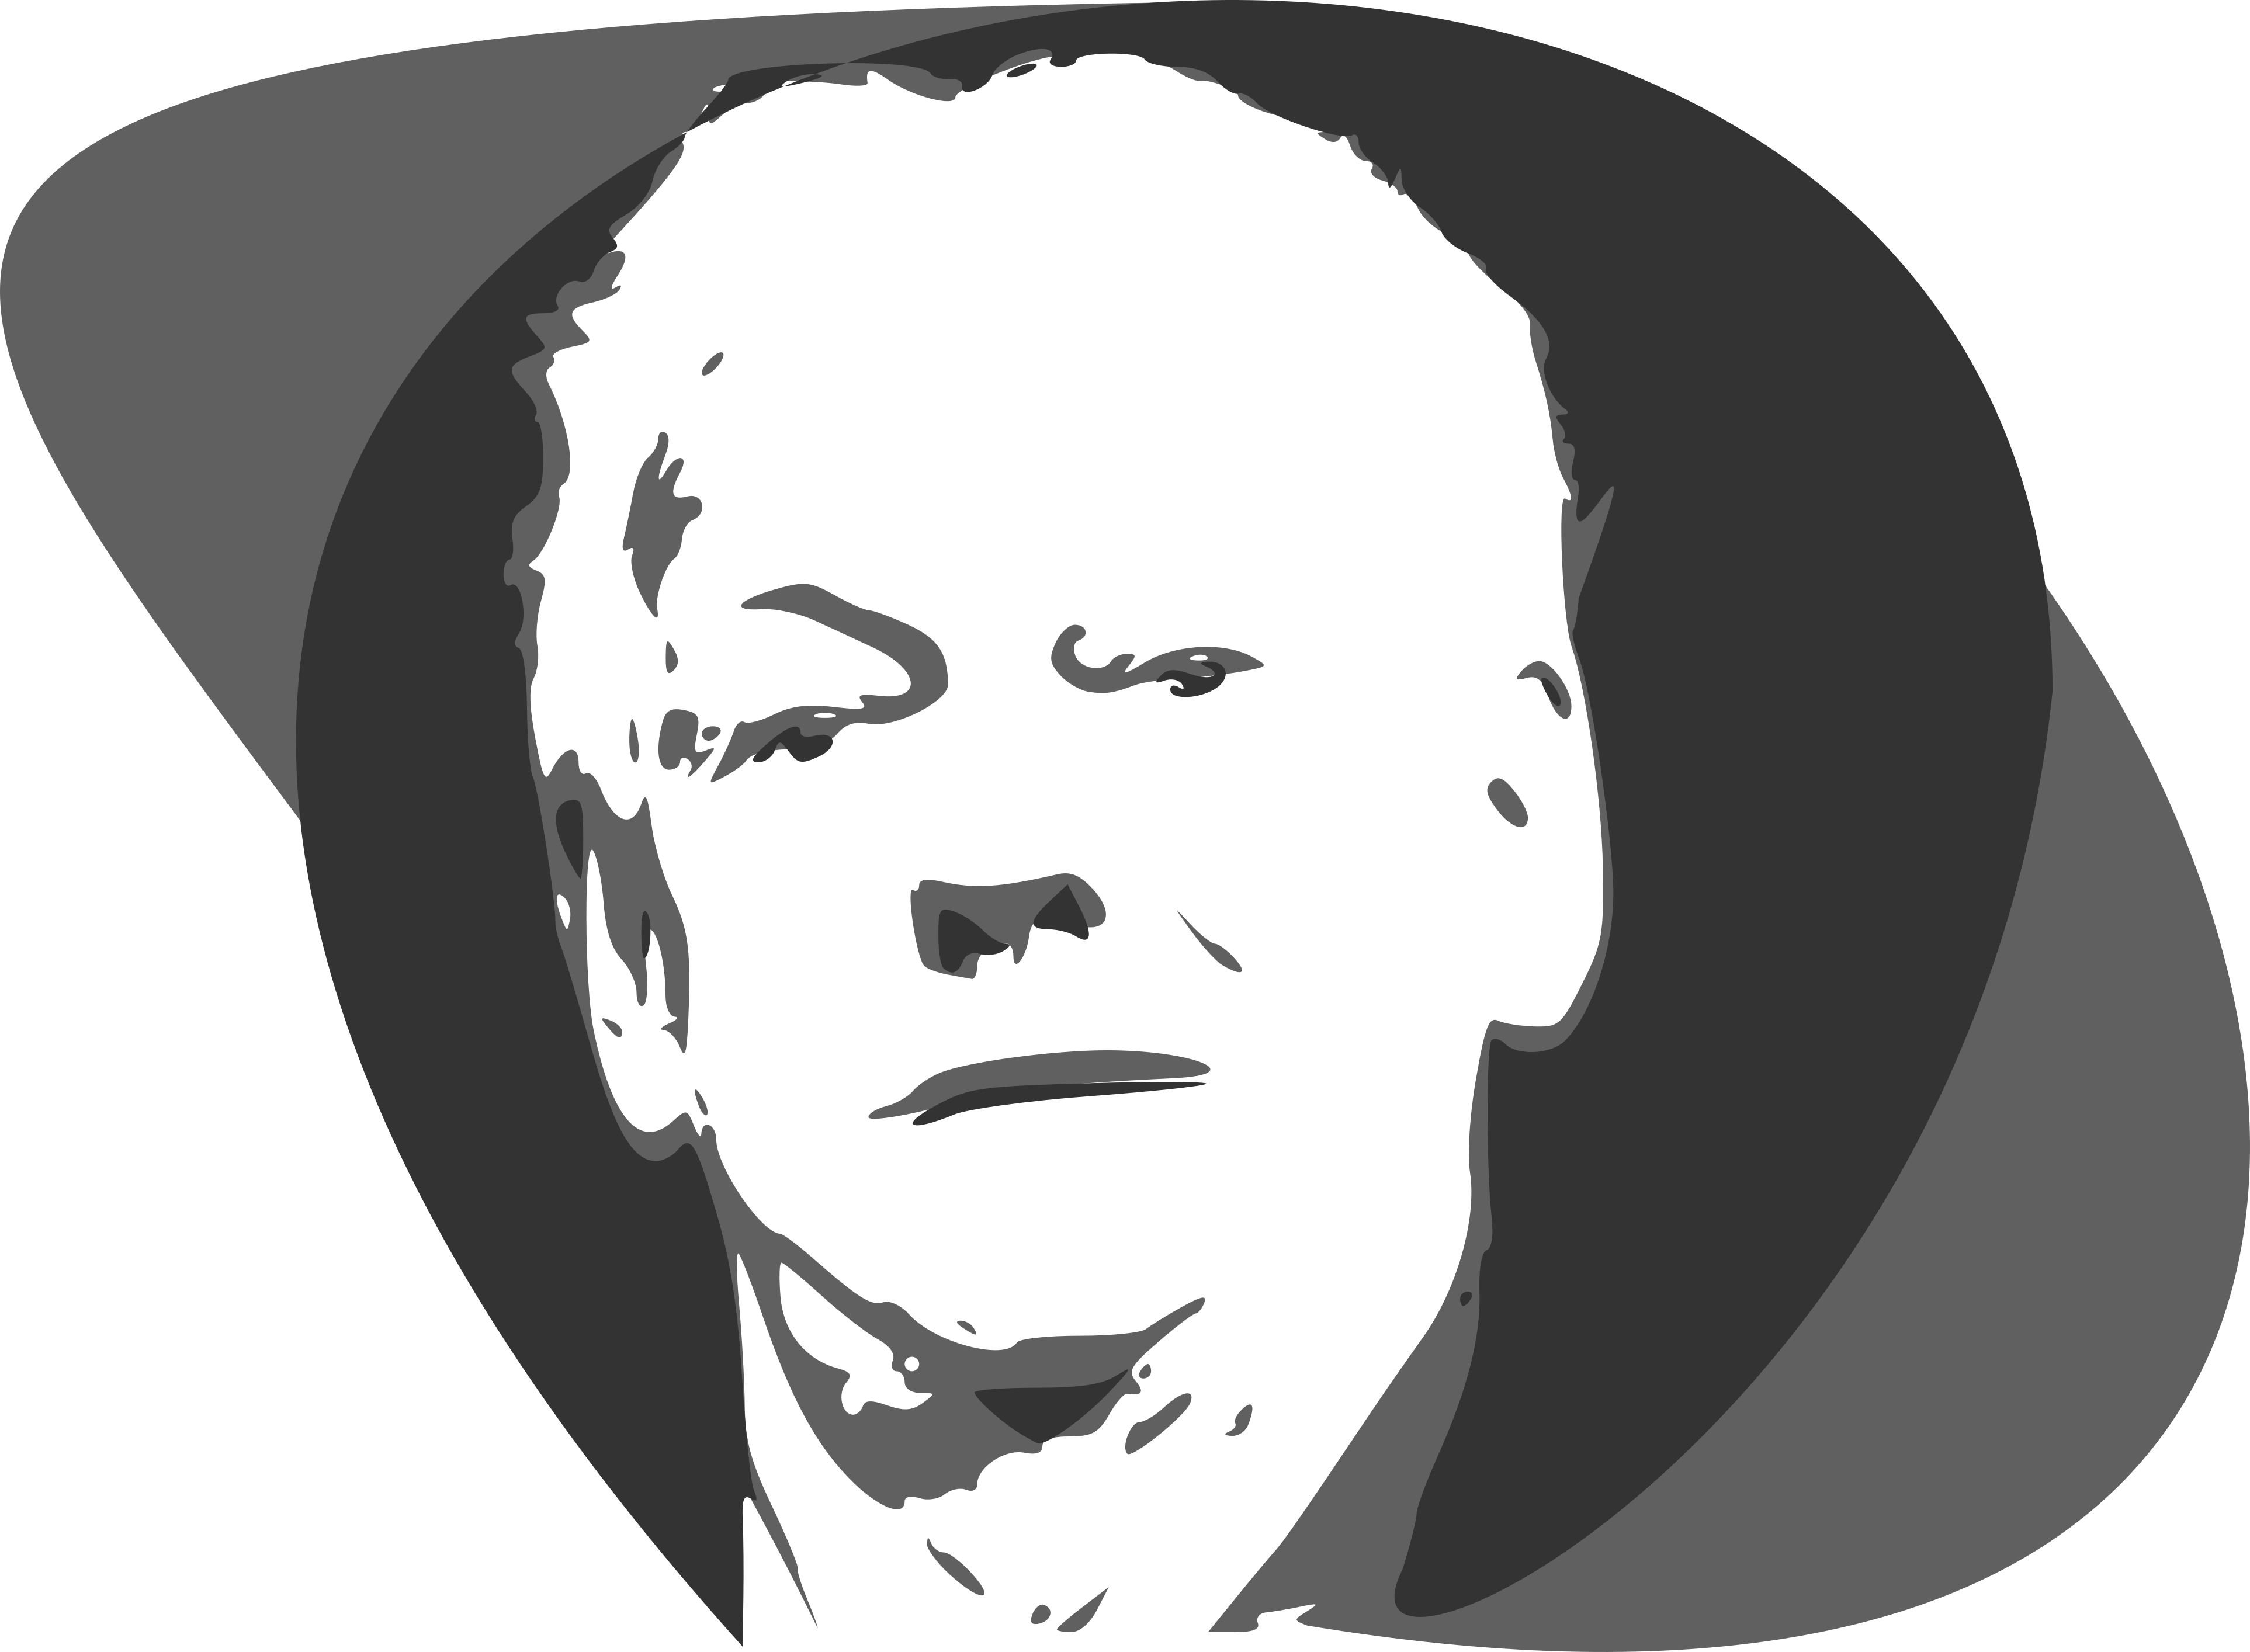
\includegraphics[width=\textwidth]{./bilder/wheterby.png}
\end{center}
\vspace*{\fill}
{\centering\fontsize{50}{48} \color{farbe}\sffamily{Wheterby Castle}\par}
\addcontentsline{toc}{chapter}{Wheterby Castle}
\newpage
%%%%%%%%%%%%%%%%%%%%%%%%%%%%%%%%%%%%%%%%%%%%%%%%%%%%%%%%%%%%%%%%%%%%%%%%%%%%%%%
\lettrine[lines=3, lhang=.2, loversize=.25, lraise=0.05, findent=0.1em,
nindent=0em]{D}{ie} Fahrt von London hat neun Stunden gedauert. Der Smog der Stadt geht fliessend in den Nebel vom Land über. Landschaft von nicht mehr als 20 Yard. Zugschwellen genen den Rythmus vor, verbieten jeden Gedanken. Tristesse und Trance im überhitzten Abteil. Von York aus nehme ich eine Kutsche in Richtung Küste. Schlaglöcher machen den Körper taub. Ich sollte für Lady Cantacuziono in London ein Stadthaus kaufen. Eine verwitwete rumänische Adlige, transsilvanischer Hochadel, sehr reich, mehr weiss ich nicht über sie. Ich habe einige Vorschläge, verschiedene Villen, ein kleines Schloss, Wohnungen in Kensington. Nachdem Geschäft sollte endlich das Gelfür die lange versprochenen Flitterwochen am Meer übrig sein. Die Hochzeit ist schon zwei Jahre her, die Erinnerung durch Alltag verblasst.

Der Kutscher bekreuzigt sich, als ich die Adresse nenne. \enquote{Seid ihr Christ? Dann nehmt dieses Kreuz.}, und reicht mir eine Kette, die fast ein Rosenkranz ist. \enquote{Das Haus ist verflucht, man sagt, dass alle die dort gewesen sind, entweder wahnsinnig wurden oder ganz verschwunden sind, überlegt es Euch gut, mein Herr.} 

Geschwätz mochte ich nie, Vorurteile kann ich mir nicht leisten. Es ist später Nachmittag als ich ankomme. Ein herrliches Schloss, historisierend gothisch, aber neu. \enquote{Sie hat einen Friedhof geschändet.} brummt der Fuhrwerker, Prim ausspuckend, brauner Schleim im Matsch. \enquote{Nun ja, nicht wirklich, aber Grabsteine für ertrunkene Seeleute haben hier gestanden, damit die Hinterbliebenen einen Ort zum Trauern haben. Ins Meer hat sie die geworfen.} Ihn ignorierend höre ich tatsächlich die See branden, tief unten an der Steilküste. Möwen schreien. Wenn ich das Meer sehe, habe ich Fernweh, schmecke Salz in der Luft. Kühler Wind, nicht stark, aber der Kraft, Armeen von Schiffen zu tragen. Mich an London erinnern, dessen Russ und Schmutz ich so liebe, ist hier unmöglich. Die Kutsche verschwindet im Nebel, mich alleine lassend.

Das schwere Tor ist geöffnet, der Garten wild, viele Rosen, in Hecken, als Büsche, rankend, blühend, verwelkt. Auf mein Klopfen reagiert niemand. \enquote{He}, rufe ich. Also stosse ich die Tür selber auf, trete ein, beklommen, ein Eindringling. Dabei sollte der Brief, der mich angekündigt hat, bereits hier sein. Ein grosser Saal, ein grosser Tisch, gedeckt für eine Person. Schweres Holz, Alter vortäuschend, als wäre es schon immer da gewesen. Gemälde bereits Verstorbener, Goldketten trangend, Zepter zur Schau stellend, Herschaflichkeit ausstrahelnd. Womit haben sie verdient, hier zu hämgen, was zeichnet sie aus?


Ein Zettel \enquote{Esst, ich stosse später zu Euch.}. Kaltes Huhn, fast roh, aber die Kartoffeln heiss und dampfend. Warum keine Bediensteten? Es ist unheimlich, ich schäme mich meiner, fühle mich falsch. Die Stille ist kaum zu ertragen. Aber die Reise war ermüdend, Hunger egalisiert anderes. Also esse ich. Der Wein ist fast schwarz, schmeckt tief und schwer, scheint sich im Hals aufzulösen, wird den Magen nie erreichen. Der beste, den ich je getrunken habe. In einem Zug leere ich den silbernen Becher, kann nicht absetzen.

\enquote{Ihr habt geschlafen.} Tatsächlich, meine Verwirrung ist vollkommen. Ich muss während des Essens eingeschlafen sein, warum erinnere ich mich an nichts? Das Huhn steht immer noch beinahe unagetastet vor mir. Es ist bereits dunkel, Kerzen erleuchten das Zimmer nur matt. Daher sehe ich sie nicht gleich, reibe mir verstört die Augen, aber noch steckt zu viel Schlaf in ihnen, um Schärfe zu erlauben.

\enquote{Willkommen auf Whetherby Castle. Ich bin Lady Cantacuziono.} Das Kreuz des Kutschers ist verschwunden, ich weiss es ohne in die Tasche zu greifen. Sie ist ganz in schwarz gekleidet, in tiefem Kontrast zu ihrer prozellanweissen Haut. Das Gesicht ist nicht zu erkennen. Seltsam langsame Bewegungen, fast verträumt. Sie nimmt eine Nuss aus einer Schale, umschliesst sie mit zarten Fingern und knackt sie, als wäre dies die natürlichste Art. Wie die Nuss in ihren Mund gelangt, verstehe ich nicht.

\enquote{Ich habe sie erwartet}. Ich stehe endlich auf, erschrocken von meiner Unhöflichkeit, verbeuge mich, gebe ihr die Hand. Wie kalt sie ist. Ich erkläre mich, stammele wie peinlich mir es sei, eingeschlafen zu sein, mit einer angedeuteten Geste deutet sie mir aufzuhören. Ich spüre wie mir Schweiss den Rücken herabläuft, bin verlegen, verunsichert.

\enquote{Wenn sie wünschen kann ich ihnen gerne die Unterlagen geben, ich habe verschiedene Optionen für sie ausgewählt\dots} 

\enquote{Sie werden mir ein Haus kaufen, ich bin an Optionen nicht interessiert.}, weist sie mich zurück. Sagt sie das wirklich oder meine ich es nur zu hören? Es muss an diesem Schlaf liegen, der nicht verschwinden will, aber warum kann ich die Frau nur undeutlich sehen? Mein Blick verschwimmt, aber nur bei Ihr. Den fetten Mann auf dem riesigen Bild sehe ich, Goldene Knöpfe auf der Brust,aber sie? Wie der Rauch einer erlöschenden Kerze.

\enquote{Erlauben sie mir eine Frage}, setze ich an, will wissen, warum es keine Diener gibt, weswegen ich mich so eigenartig fühle, aber sie verneint bevor ich die Frage stellen kann mit einer Geste, die ich nicht kenne aber verstehe. Pachuli. Ein schwerer Geruch umströmt sie, wird mir jetzt bewusst, erreicht mich, dringt auch in mich ein. Ich muss endlich aufhören zu träumen, muss mich fokussieren, kann es aber nicht. Werde immer tiefer hinabgezogen. Sand zerrieselt zwischen meinen Fingern. Ich entschuldige mich stotternd, versuche die Fassung zu wahren. War sie eben auch schon so riesig? Sie scheint den Raum vollständig auszufüllen, ist dabei aber weiter zerbrechlich zart, elegant. Ihr Anblick verweht, wenn ich ihn fassen will, sie ist überall und doch nicht da. Ich spüre ihre glatte und zarte Haut.

Ich stütze mich auf den Tisch, der Schweiss tropft mir aus den Haaren, wie finde ich mich wieder? Sie führt mich in ein Zimmer, ich schlottere, kann mir nicht helfen. Dass sie mir zwei riesige Hunde zu meinem Schutz da lässt, nehme ich nicht wahr. Gross und drohend sitzen sie vor meinem Bett, in das ich sinke ohne die Kleider zu wechseln. Sie werden die ganze Nacht knurren und am Morgen verschwunden sein. Ich schlafe nicht, träume nur. Der einzige Mitgefangene in meinem kleinen Kerker ist meine Angst. Schwarz und kalt. Einsamkeit, Verlassensein, Leere. Als endlich die Sonne aufgeht stehe ich auf, bin wieder alleine in dem Schloss. Die Nacht ist vorbei, ich weiss wieder wer ich bin, was ich bin. 

Ein unterschriebener Kaufvertrag liegt auf dem Tisch, von draussen ruft ein Kutscher.\hfill \pgfornament[color=farbe,height=.5cm]{3}
\newpage 

%%%%%%%%%%%%%%%%%%%%%%%%%%%%%%%%%%%%%%%%%%%%%%%%%%%%%%%%%%%%%%%%%%%%%%%%%%%%%%%%%%%%%%%%%%%%%%%%%%%%%%
%Inhaltsverzeichnis
\newpage
\pagestyle{empty}
\tableofcontents

\end{document}
